\documentclass{article}

\usepackage[utf8]{inputenc}
% \usepackage[english,greek]{babel}
\usepackage[unicode]{hyperref}
\usepackage[LGR, T1]{fontenc}
\usepackage{amsfonts, alphabeta, amssymb}
\usepackage[none]{hyphenat}
\usepackage{amsmath, slashed, graphicx, physics, tikz, braket, caption, subfig, comment, geometry, multicol, lipsum, fancyhdr, tcolorbox, siunitx, authblk, xcolor, abstract, float, indentfirst, xfrac, cancel, bbold, appendix, tikz, tikz-feynman, tensor, multirow, makecell, algpseudocode, algorithmicx, algorithm, changepage, adjustbox, lscape, placeins, xcolor, listings}
% \usepackage[style=numeric-comp,sorting=none]{biblatex}
% \setcounter{secnumdepth}{3}
% \setcounter{tocdepth}{3}
\title{
        \textbf{Study of a new kinematic weighting algorithm for the measurement of CP asymmetries in charm decays}
        \\
        LHCb Collaboration
}
\author{Georgios Christou}
\date{
        $6^{th}$ Week
        \\
        17/07/2023 - 21/07/2023
}

\begin{document}
    \begin{figure}[t]
        \centering
        \subfloat{
\includegraphics[height = 3.5cm]{../../.images/CERN_logo.png}}
        \hspace{1cm}
        \subfloat{
\includegraphics[height = 3.5cm]{../../.images/Lhcb-logo-new.svg.png}}
    \end{figure}
    \maketitle

    \pagebreak
    
    \section{Introduction}

    We use a high statistics sample to calculate more accurately the weighting function which is given by
    \begin{equation}
        \label{eq:weighting}
        Q(\vec{p}_{D^\star}, \vec{p}_{\pi_s}) \simeq \frac{\Gamma_{D^0}^{\pi\pi}(\vec{p}_{D^\star} - \vec{p}_{\pi_s}) + \Gamma_{\bar{D}^0}^{\pi\pi}(\vec{p}_{D^\star} - \vec{p}_{\pi_s})}{\Gamma_{D^0}^{KK}(\vec{p}_{D^\star} - \vec{p}_{\pi_s}) + \Gamma_{\bar{D}^0}^{KK}(\vec{p}_{D^\star} - \vec{p}_{\pi_s})}
    \end{equation}

    \begin{figure}[h!]
        \centering
        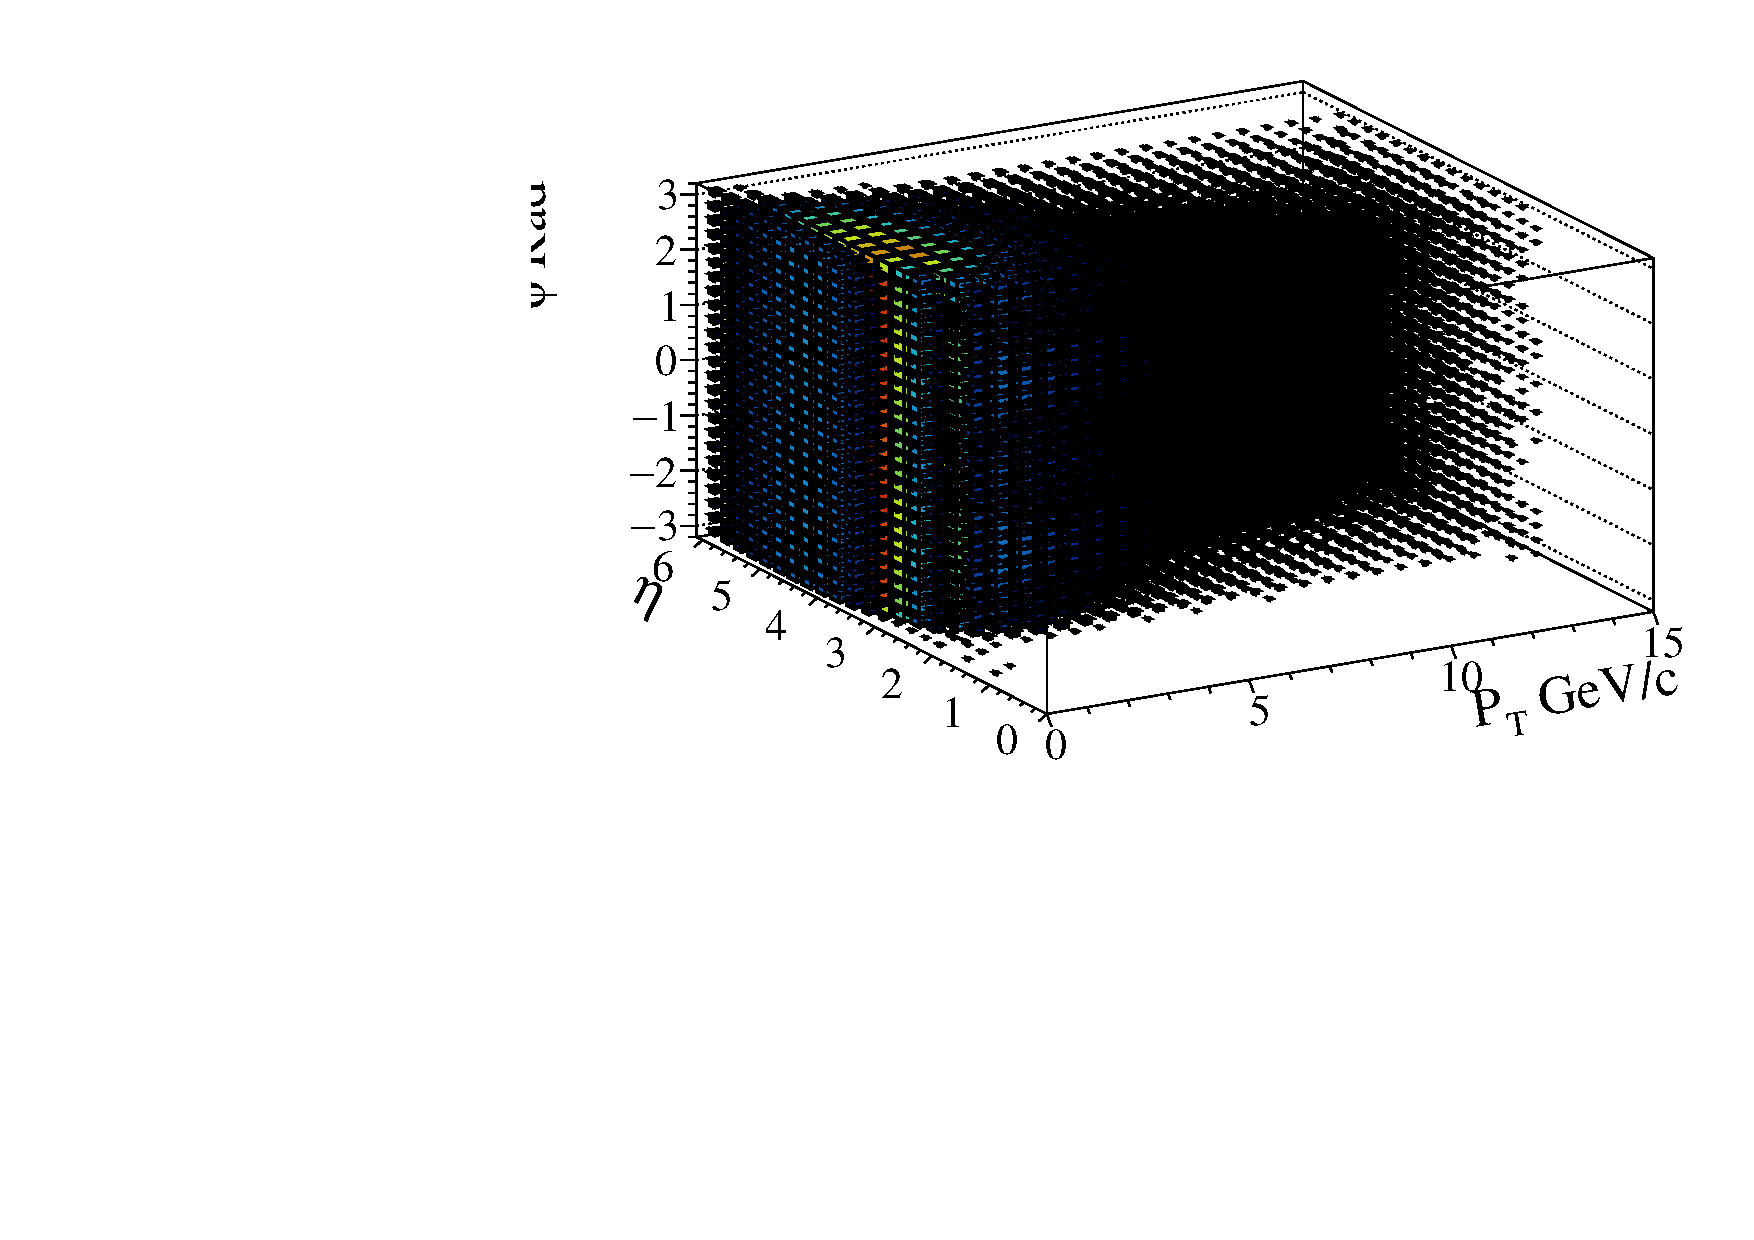
\includegraphics[width = 0.7\textwidth]{../../work/RapidSimAnalysis/WeightingFunction/Plots/KmKpNormalizedDistribution.pdf}
        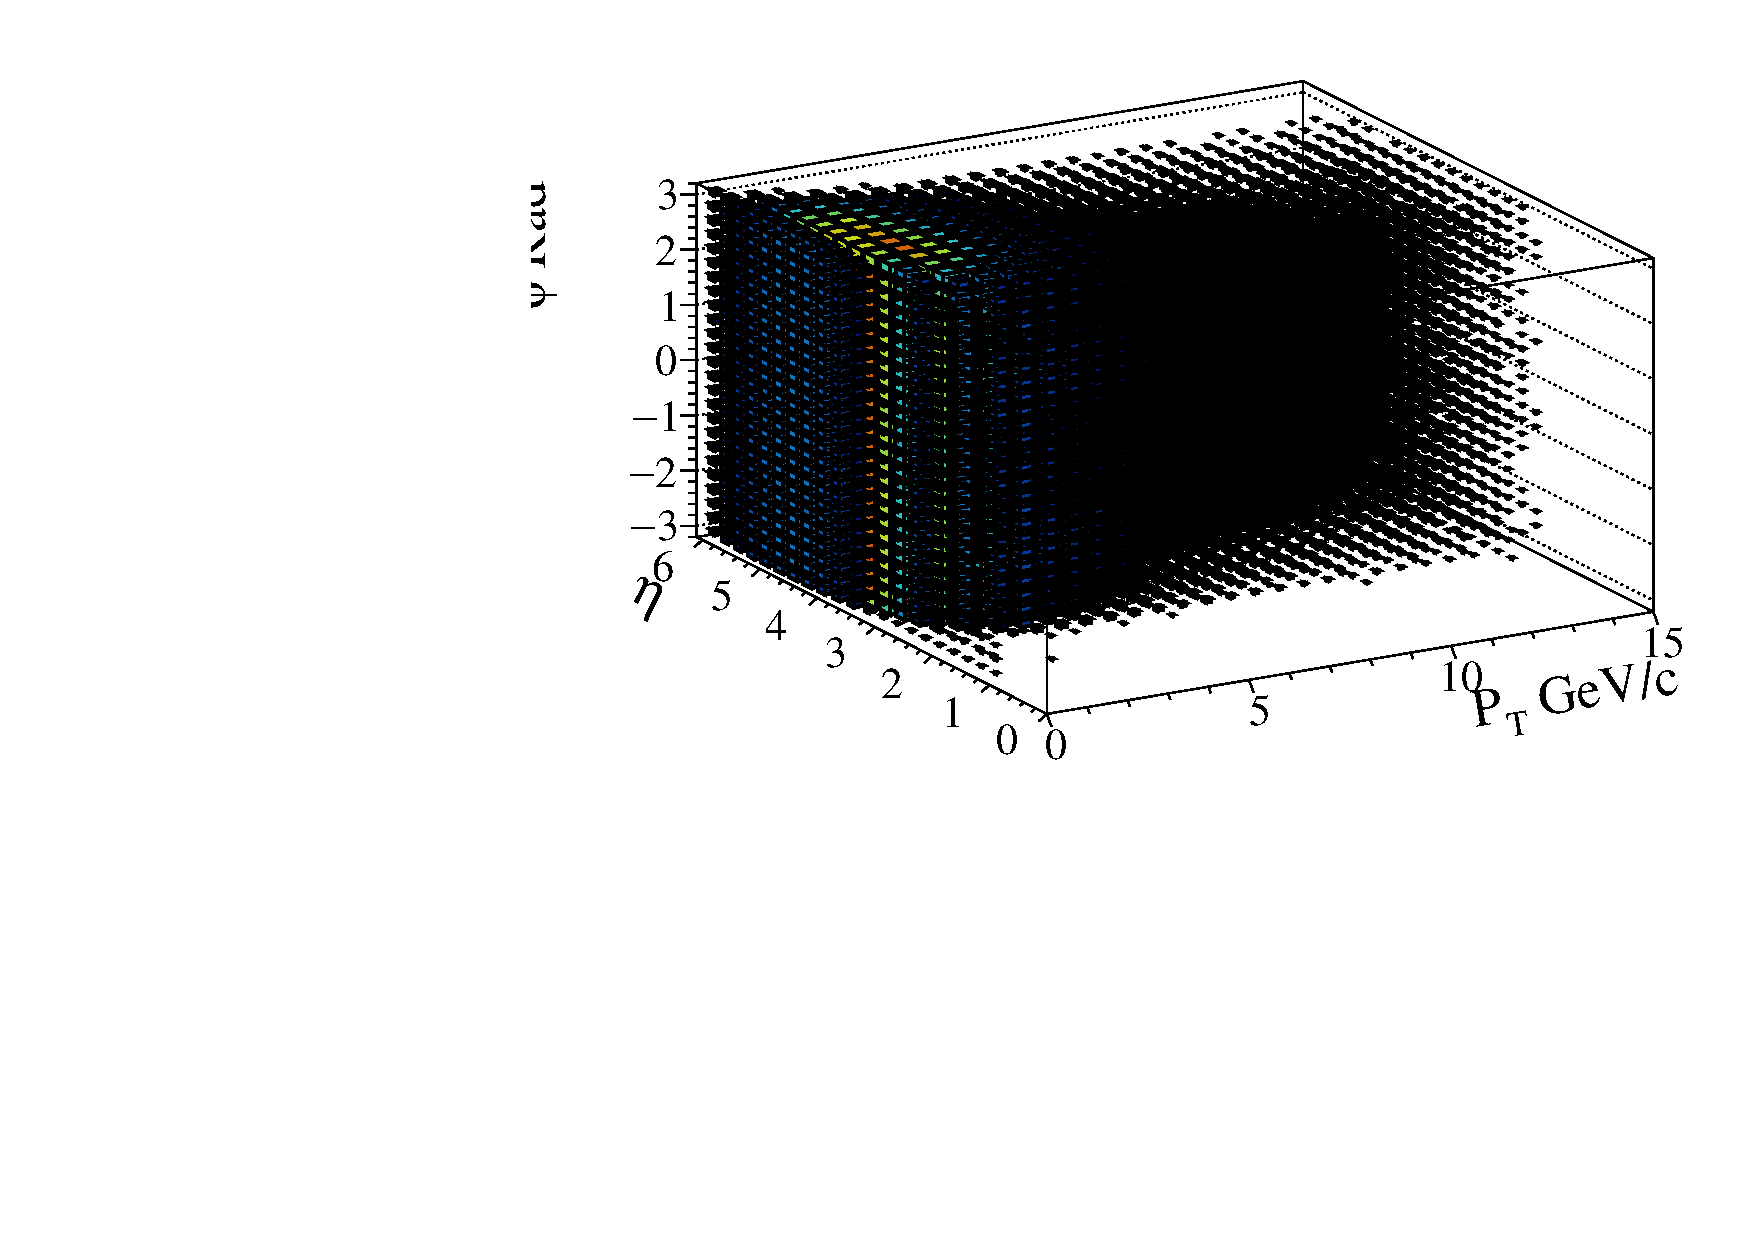
\includegraphics[width = 0.7\textwidth]{../../work/RapidSimAnalysis/WeightingFunction/Plots/pimpipNormalizedDistribution.pdf}
        \caption{Normalized distributions for $D^0\to K^-K^+$ (top) and $D^0\to \pi^-\pi^+$ (bottom).}
    \end{figure}

    Using the weighting function Eq. \ref{eq:weighting} we assign weights to the low statistics $D^0 \to K^-K^+$ sample, thus, we equalize the kinematic distributions of $D^0$.

    \begin{figure}[h!]
        \centering
        \subfloat{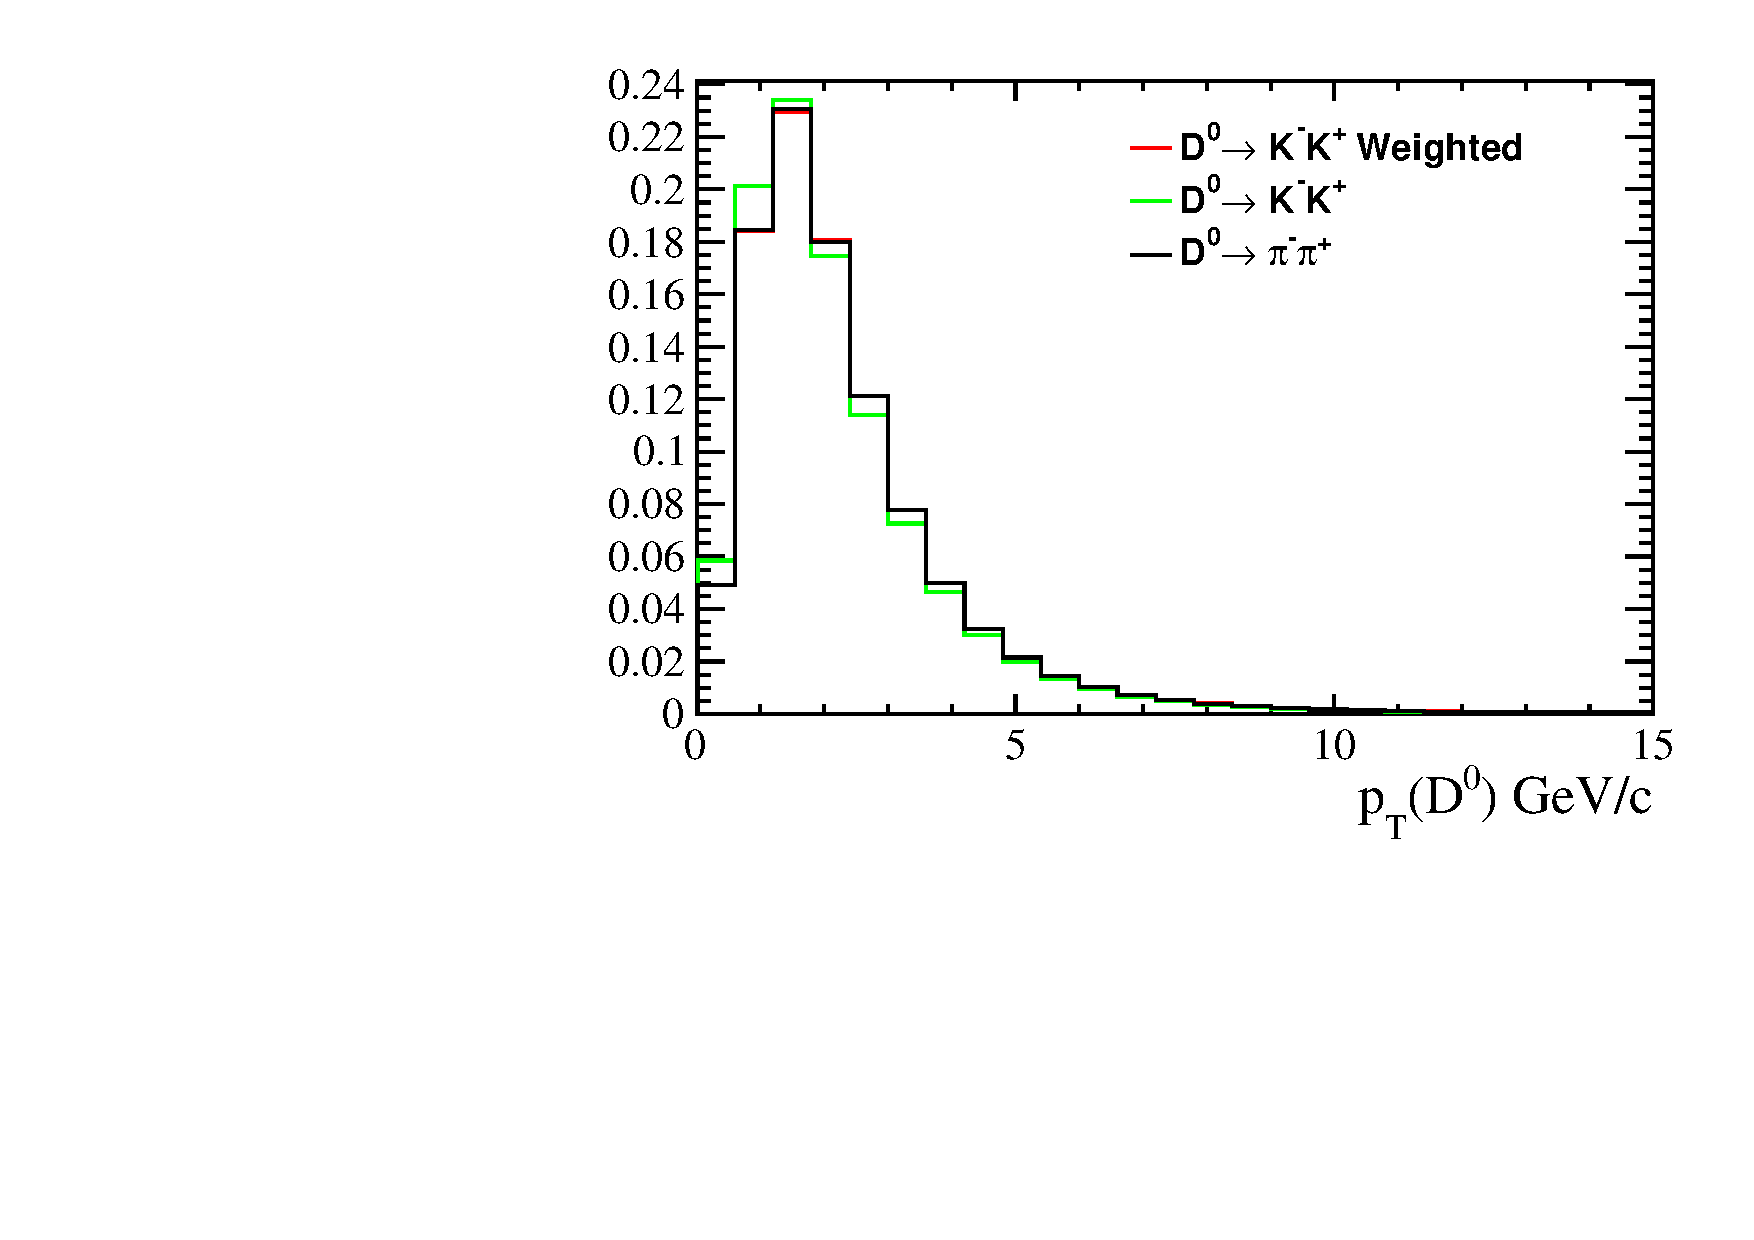
\includegraphics[width = 0.5\textwidth]{../../work/RapidSimAnalysis/WeightingFunction/Plots/D0_PT_All.pdf}}
        \subfloat{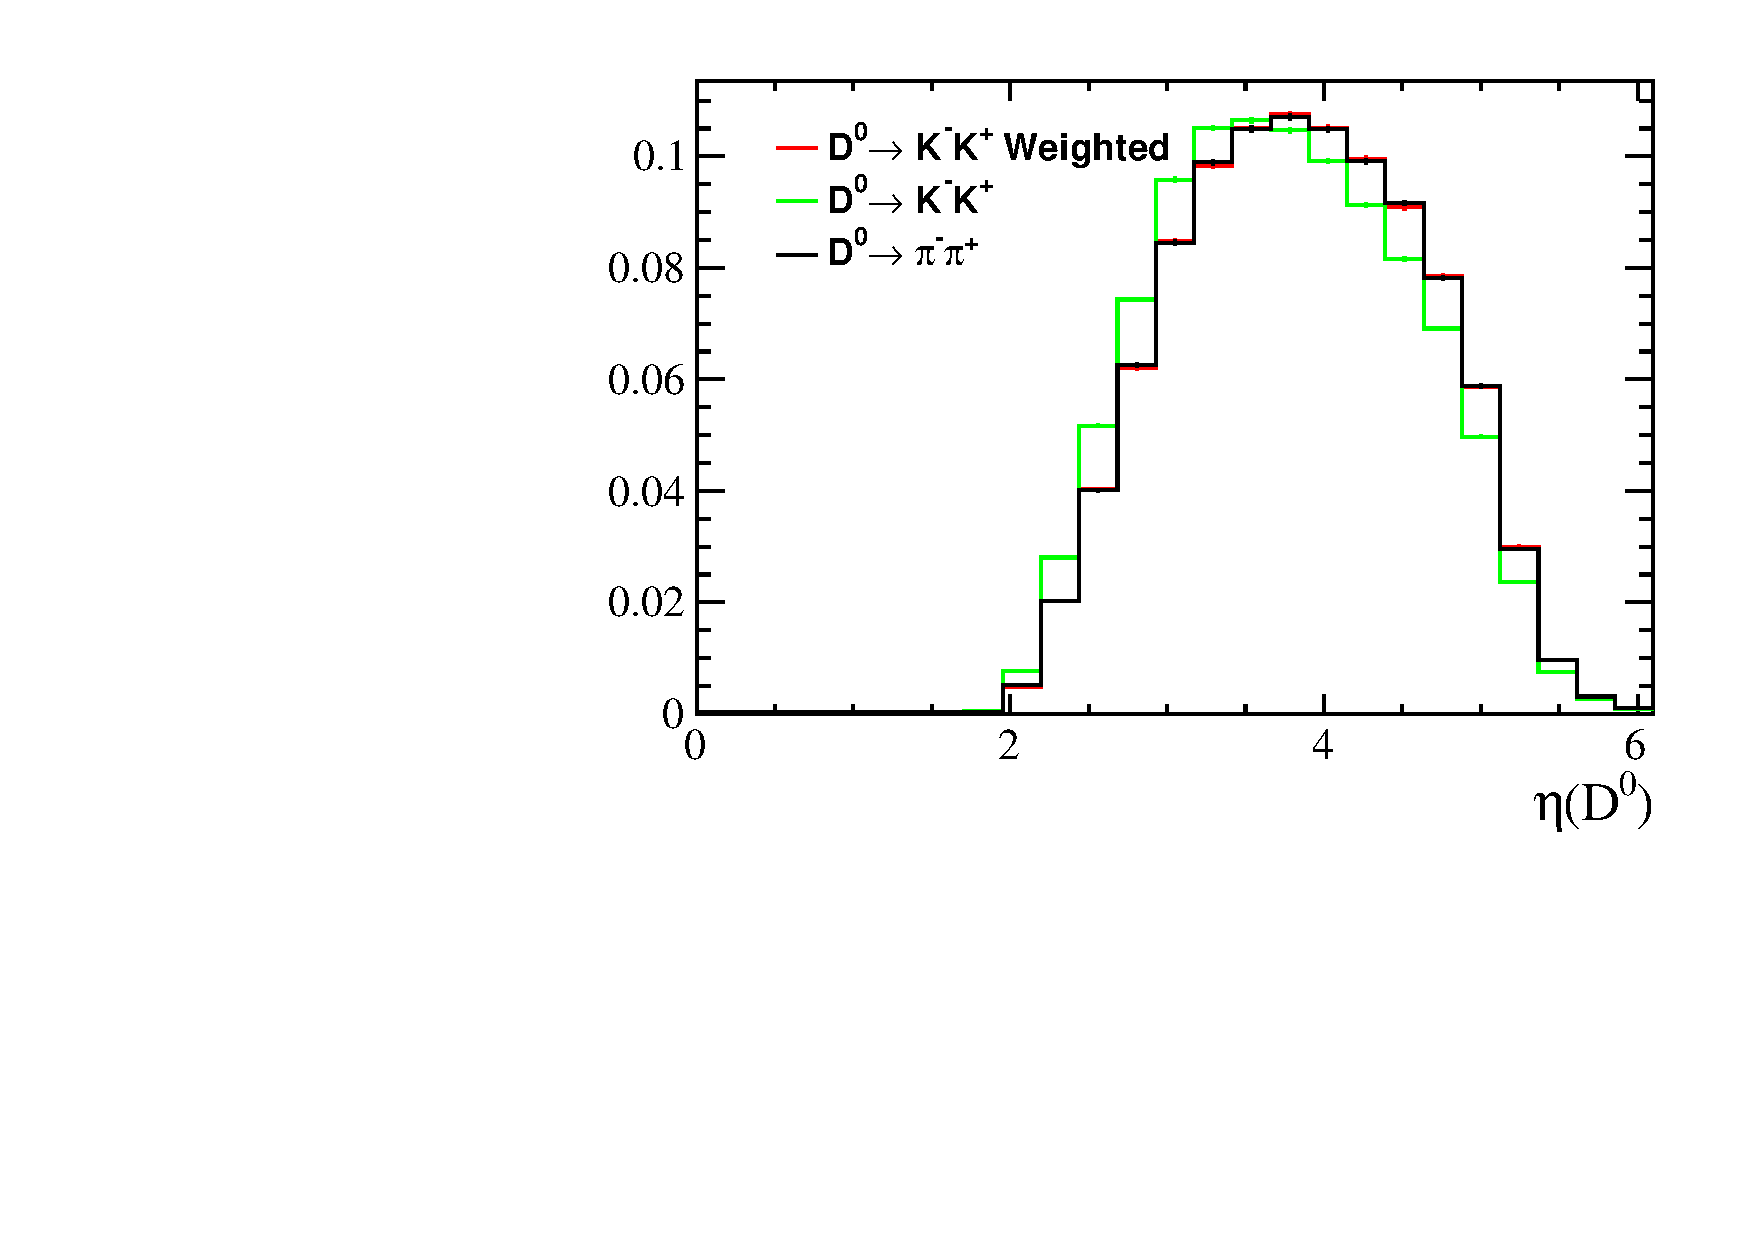
\includegraphics[width = 0.5\textwidth]{../../work/RapidSimAnalysis/WeightingFunction/Plots/D0_eta_All.pdf}}
        \hfill
        \subfloat{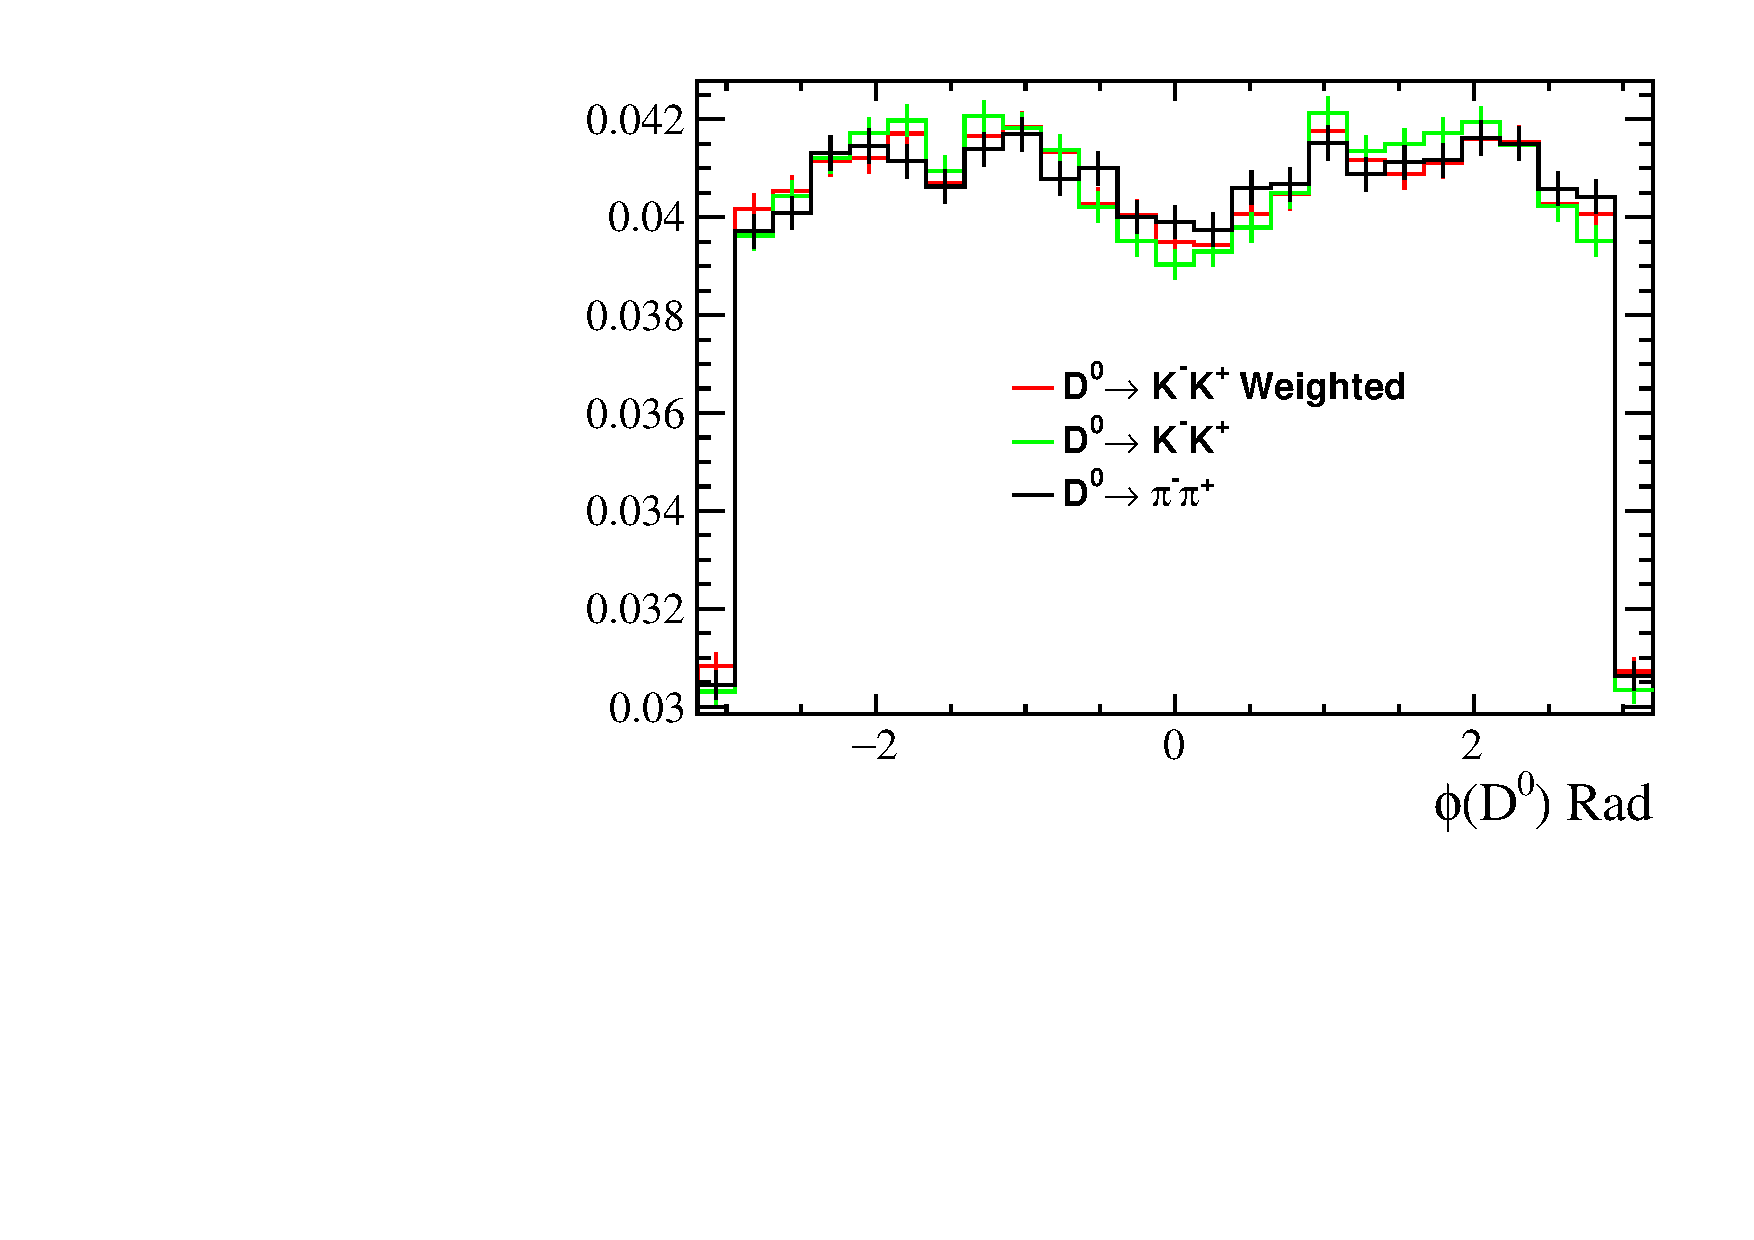
\includegraphics[width = 0.5\textwidth]{../../work/RapidSimAnalysis/WeightingFunction/Plots/D0_phi_All.pdf}}

        \caption{We present the kinematic distributions $p_T$, $\eta$ and $\phi$ of $D^0$ for the two decay modes, before and after weighting.}
    \end{figure}

    We can compare how the total asymmetry is affected.
    The total asymmetry can be measured using
    \begin{equation}
        A_{\text{total}} = \frac{N^+ - N^-}{N^+ + N^-}
    \end{equation}
    and the error can be estimated using the standard error propagation
    \begin{equation}
        \sigma A_{\text{total}} ^2 = \left(\pdv{A_{\text{total}}}{N^+}\sigma N^+\right)^2 + \left(\pdv{A_{\text{total}}}{N^-}\sigma N^-\right)^2
    \end{equation}
    For the weighted sample, $N^{\pm} = \sum_i w^\pm_i$ and $\sigma N^\pm = \sqrt{\sum_i w_i^\pm}$

    \begin{center}
        \begin{tabular}{c|c|c}
             & Weighted & Unweighted\\
             \hline\hline
            $A_{\text{total}}$ & $0.1517 \pm 0.0020$ & $0.1647 \pm 0.0020$\\
        \end{tabular}
        \captionof{table}{Total asymmetry for $D^0\to K^-K^+$ sample with and without weights.}
    \end{center}

    For the $D^0\to \pi^-\pi^+$ sample the total calculated asymmetry is
    \begin{equation}
        A_{\text{total}} = 0.2446 \pm 0.0021
    \end{equation}

    Furthermore, we compare the kinematics of $D^\star$ and $\pi_s$ to see whether or not the distributions are equalized after the weighting.

    \begin{figure}[h!]
        \centering
        \subfloat{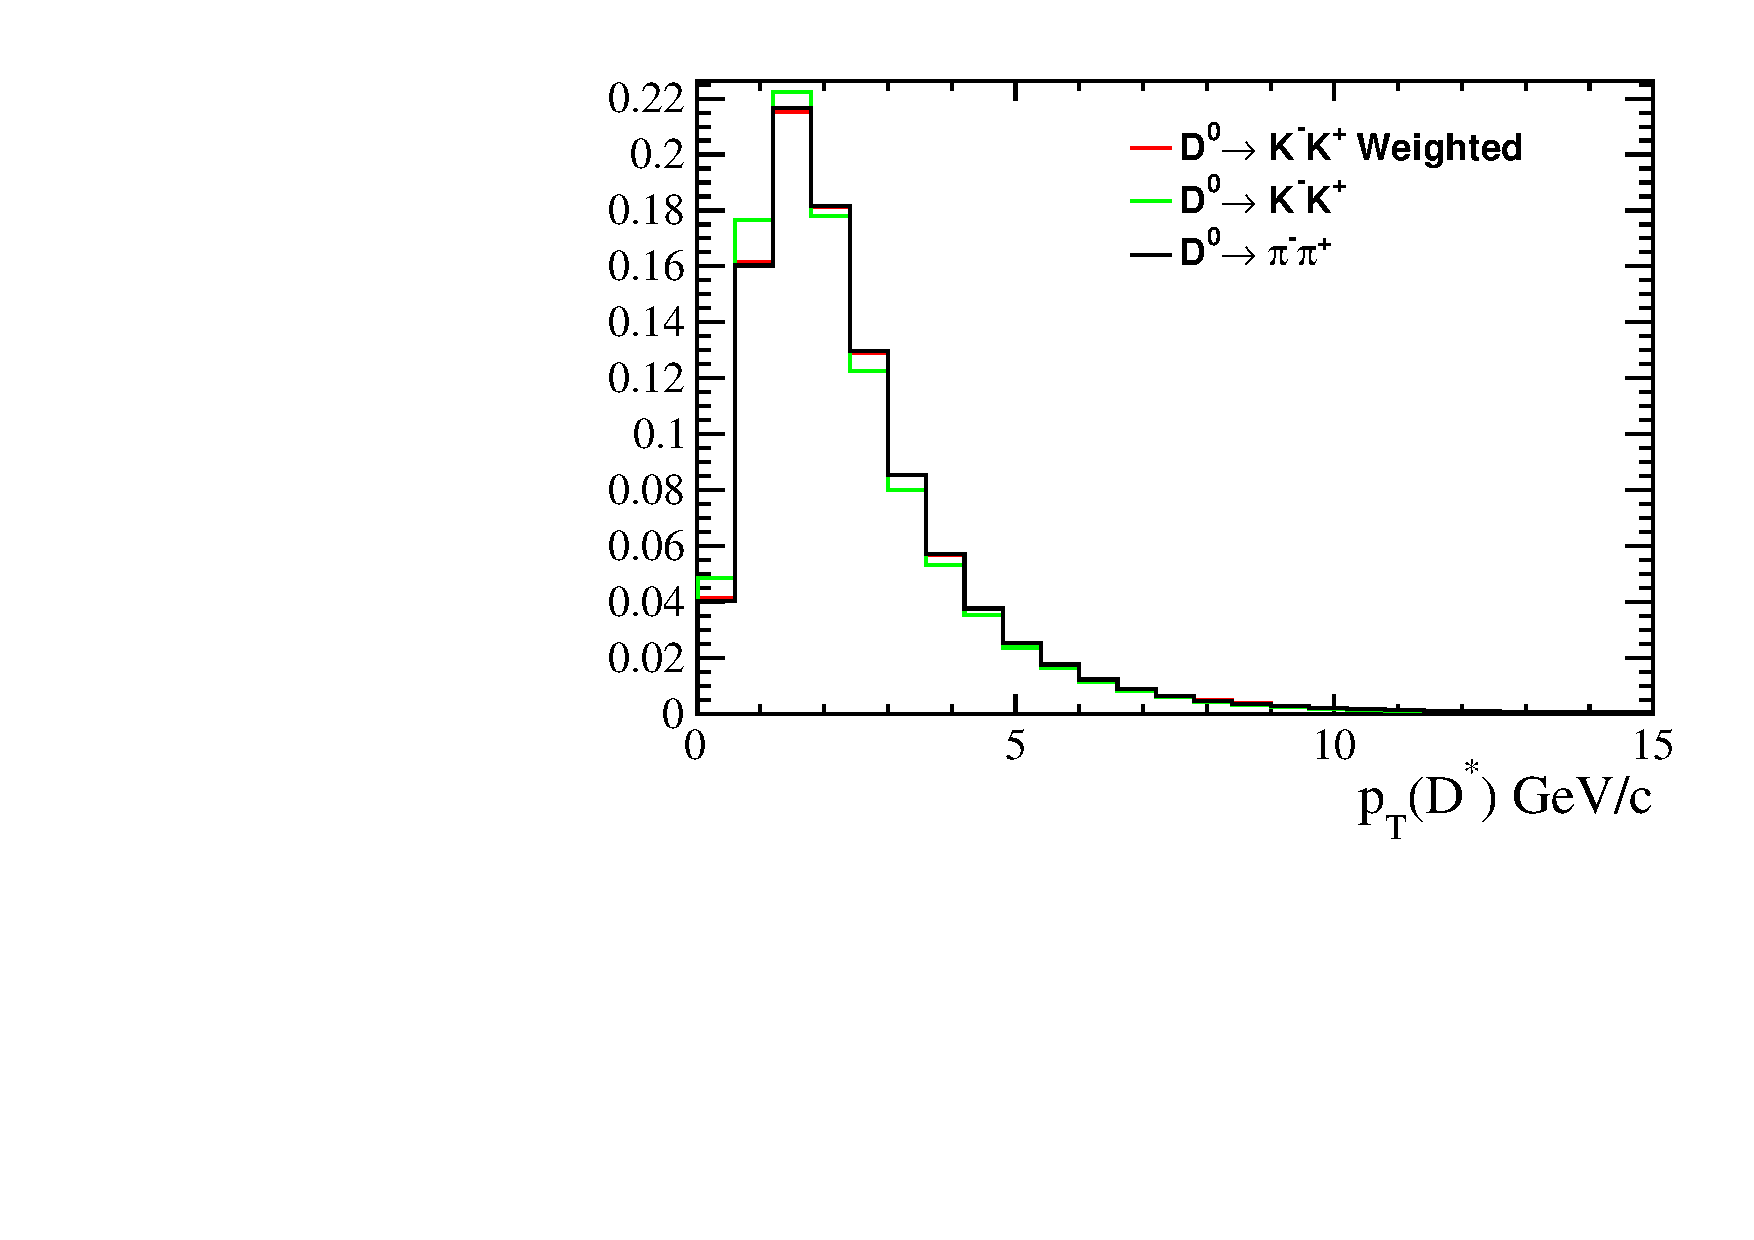
\includegraphics[width = 0.5\textwidth]{../../work/RapidSimAnalysis/WeightingFunction/Plots/Dst_PT_All.pdf}}
        \subfloat{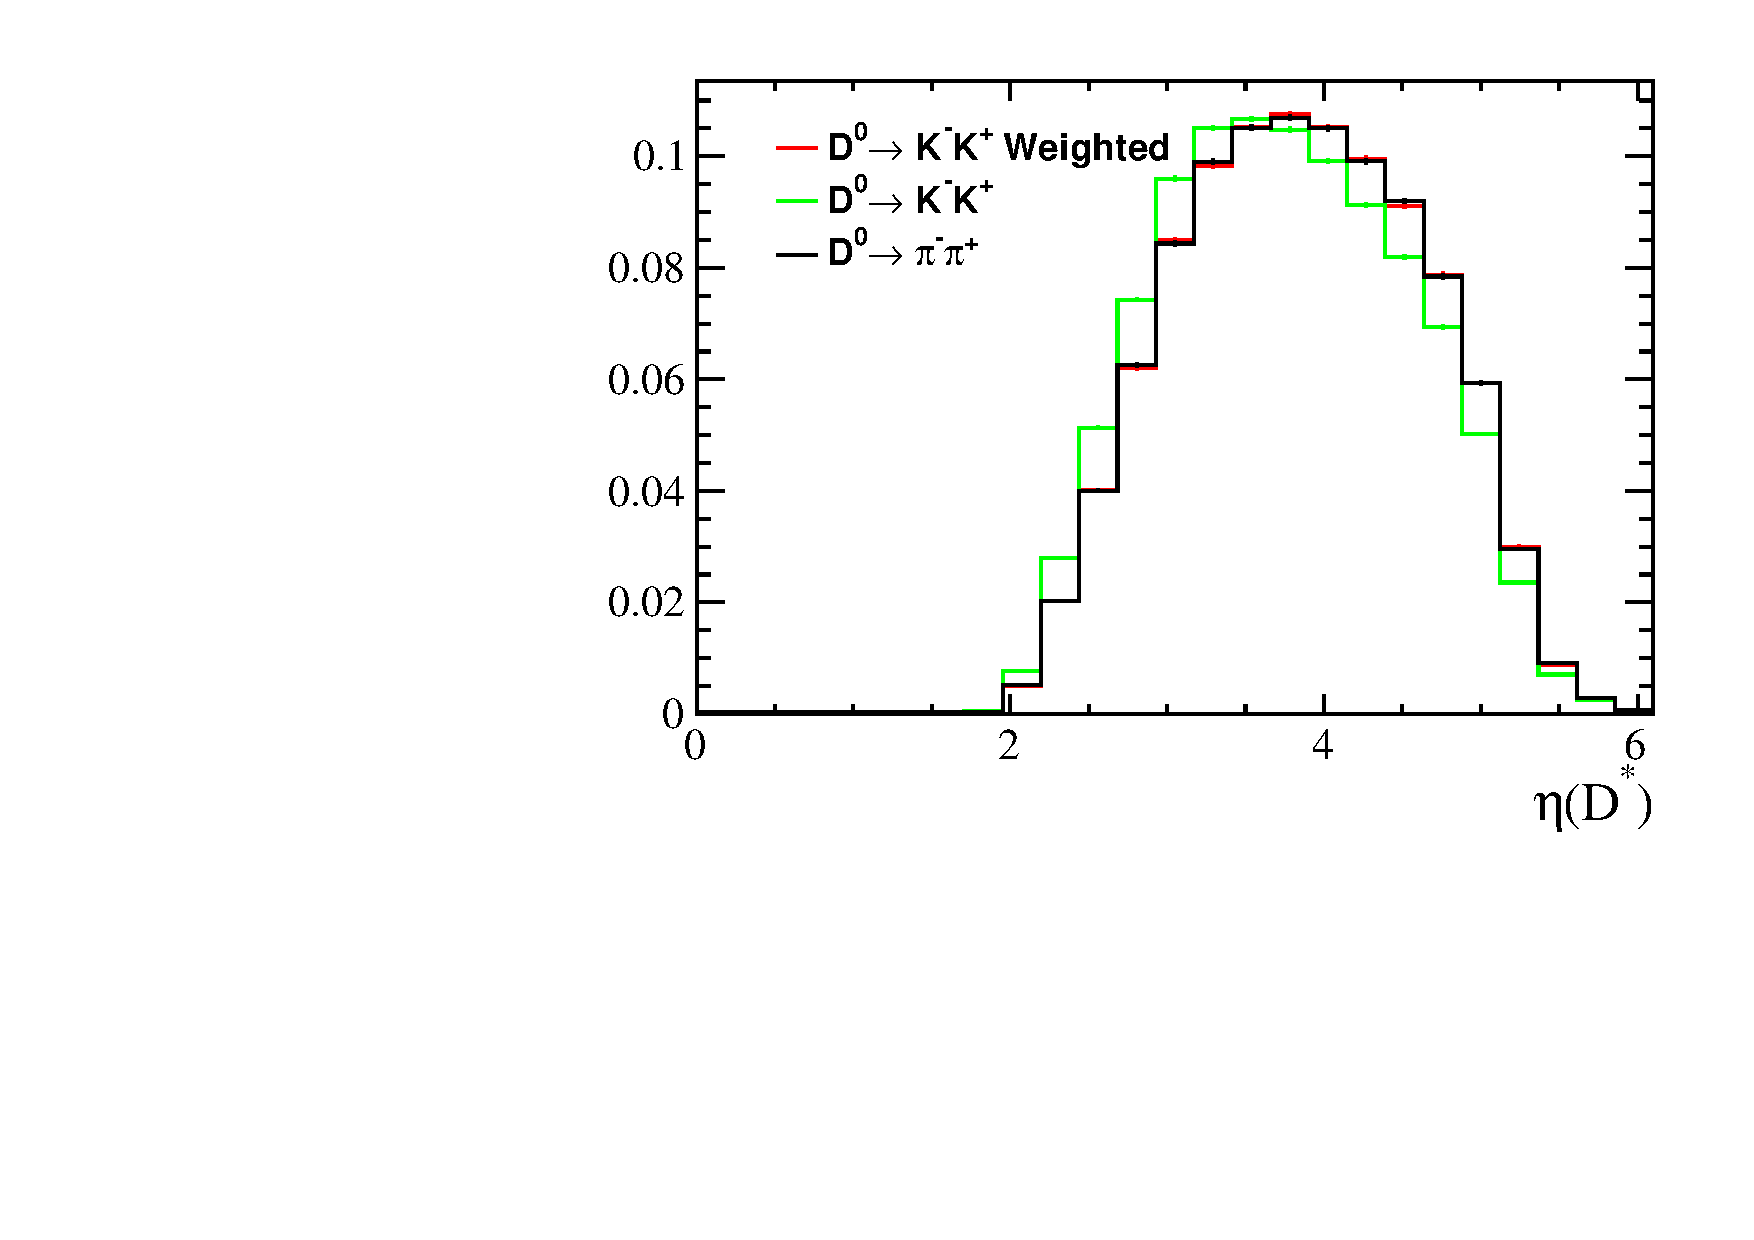
\includegraphics[width = 0.5\textwidth]{../../work/RapidSimAnalysis/WeightingFunction/Plots/Dst_eta_All.pdf}}
        \hfill
        \subfloat{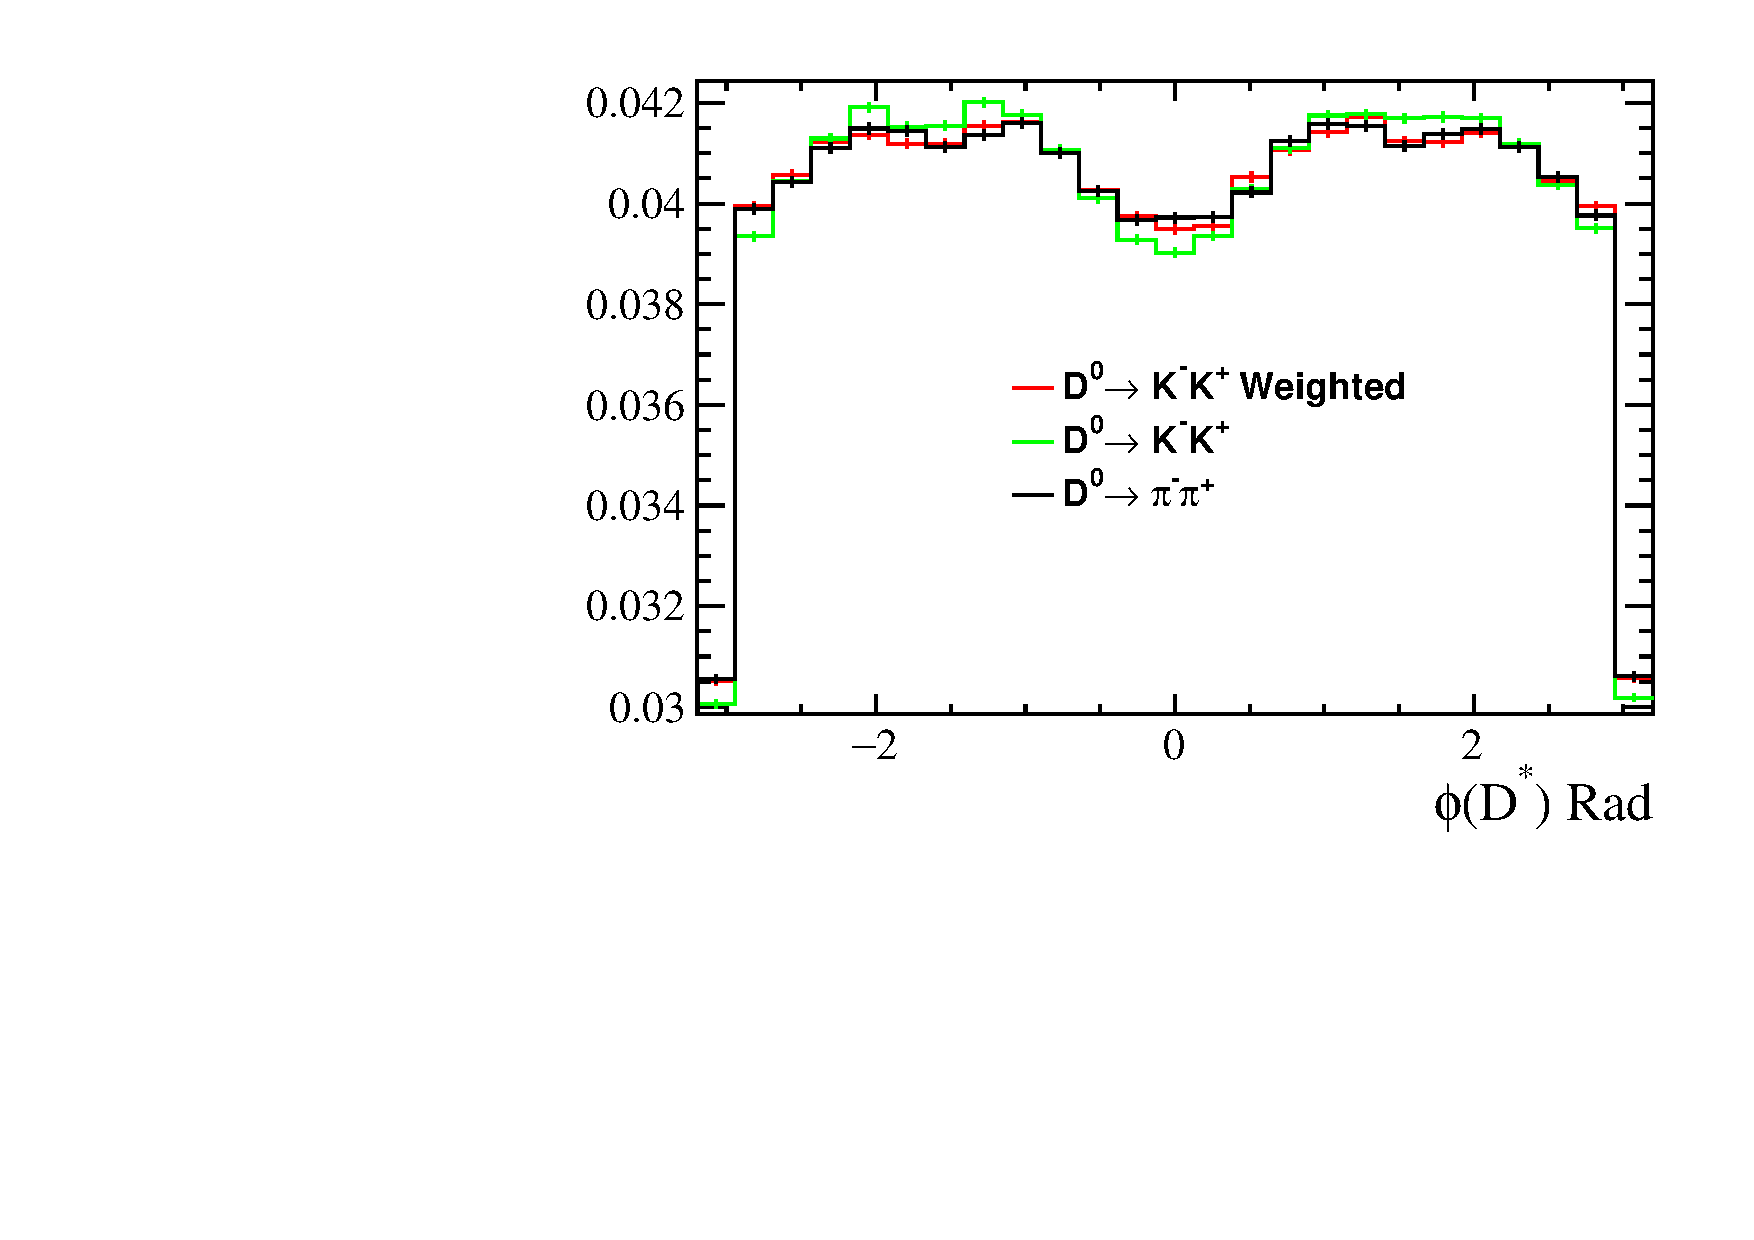
\includegraphics[width = 0.5\textwidth]{../../work/RapidSimAnalysis/WeightingFunction/Plots/Dst_phi_All.pdf}}
        \caption{We present the kinematic distributions $p_T$, $\eta$ and $\phi$ of $D^\star$ for the two decay modes, before and after weighting.}
    \end{figure}
    \begin{figure}[h!]
        \centering
        \subfloat{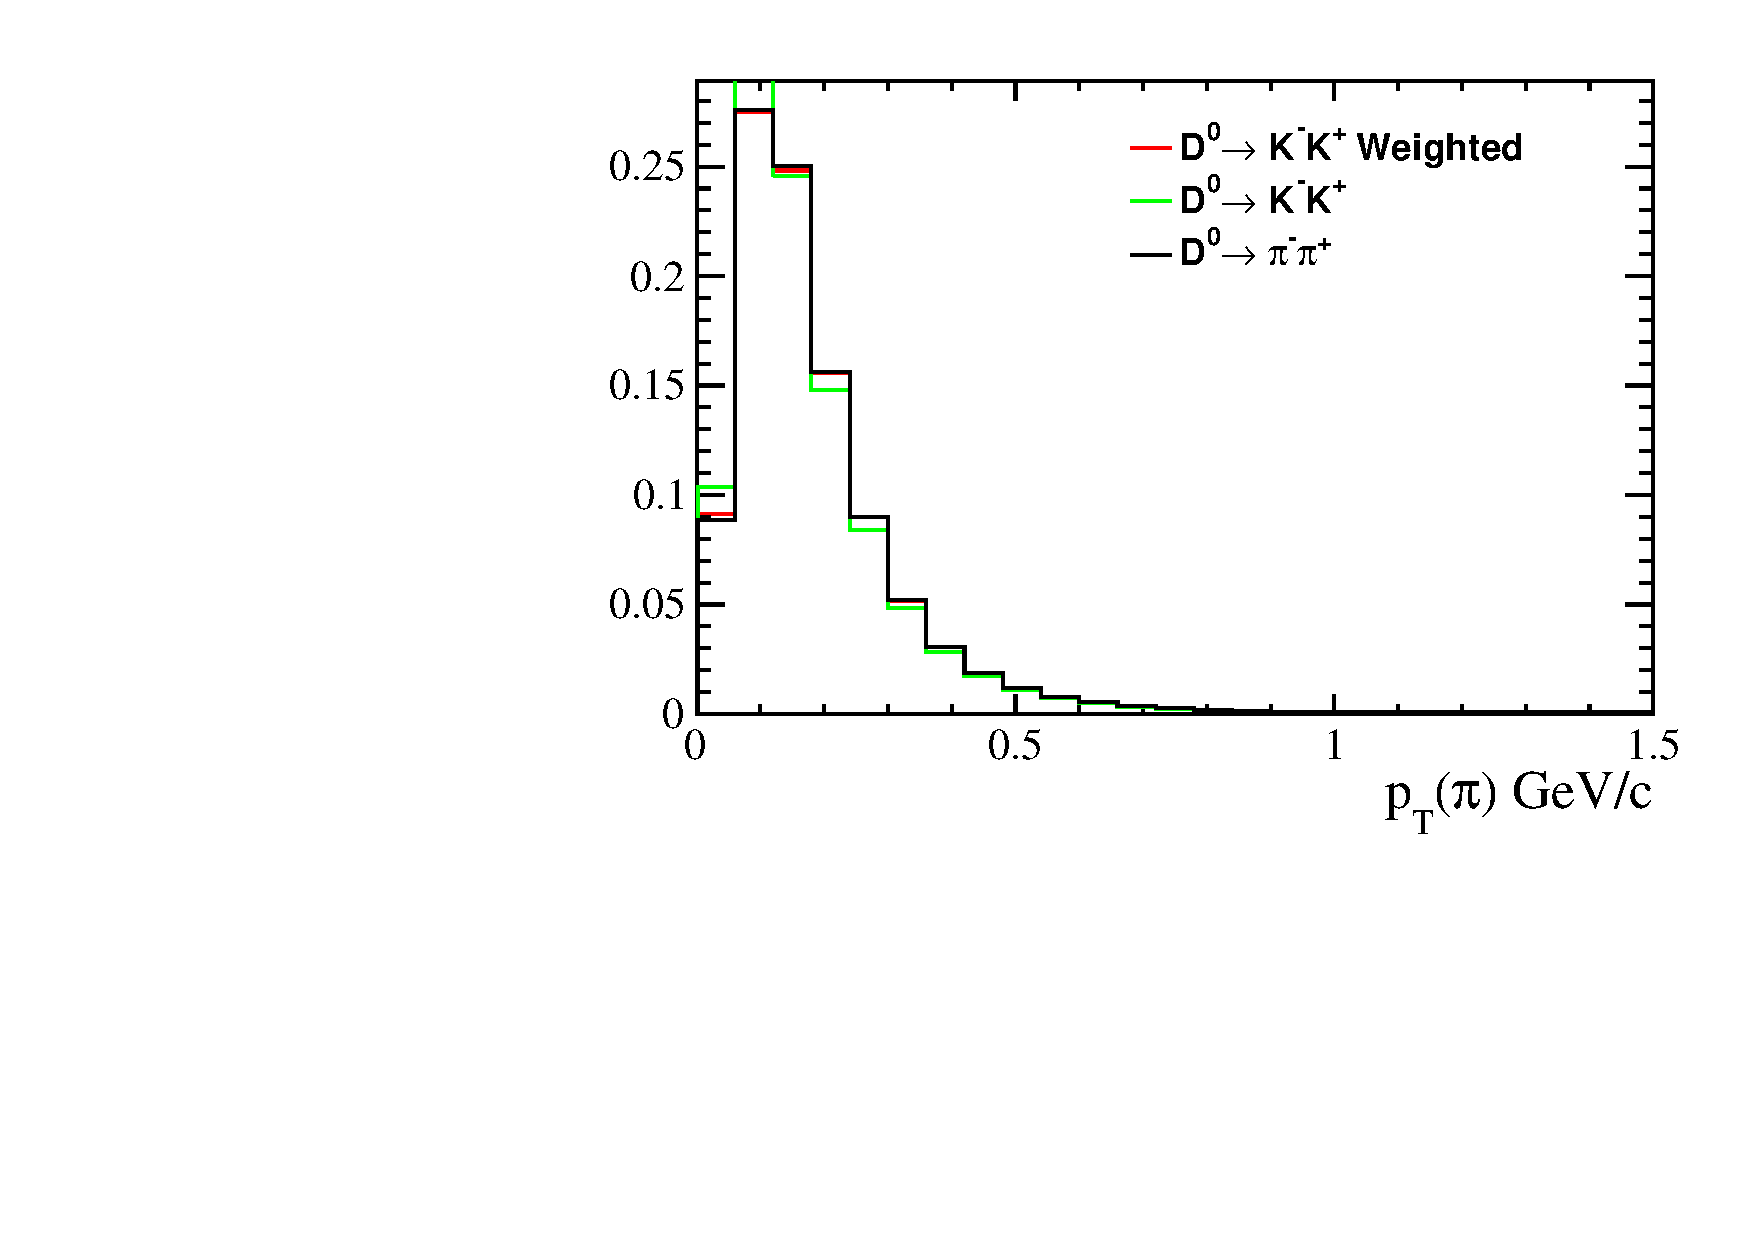
\includegraphics[width = 0.5\textwidth]{../../work/RapidSimAnalysis/WeightingFunction/Plots/sPi_PT_All.pdf}}
        \subfloat{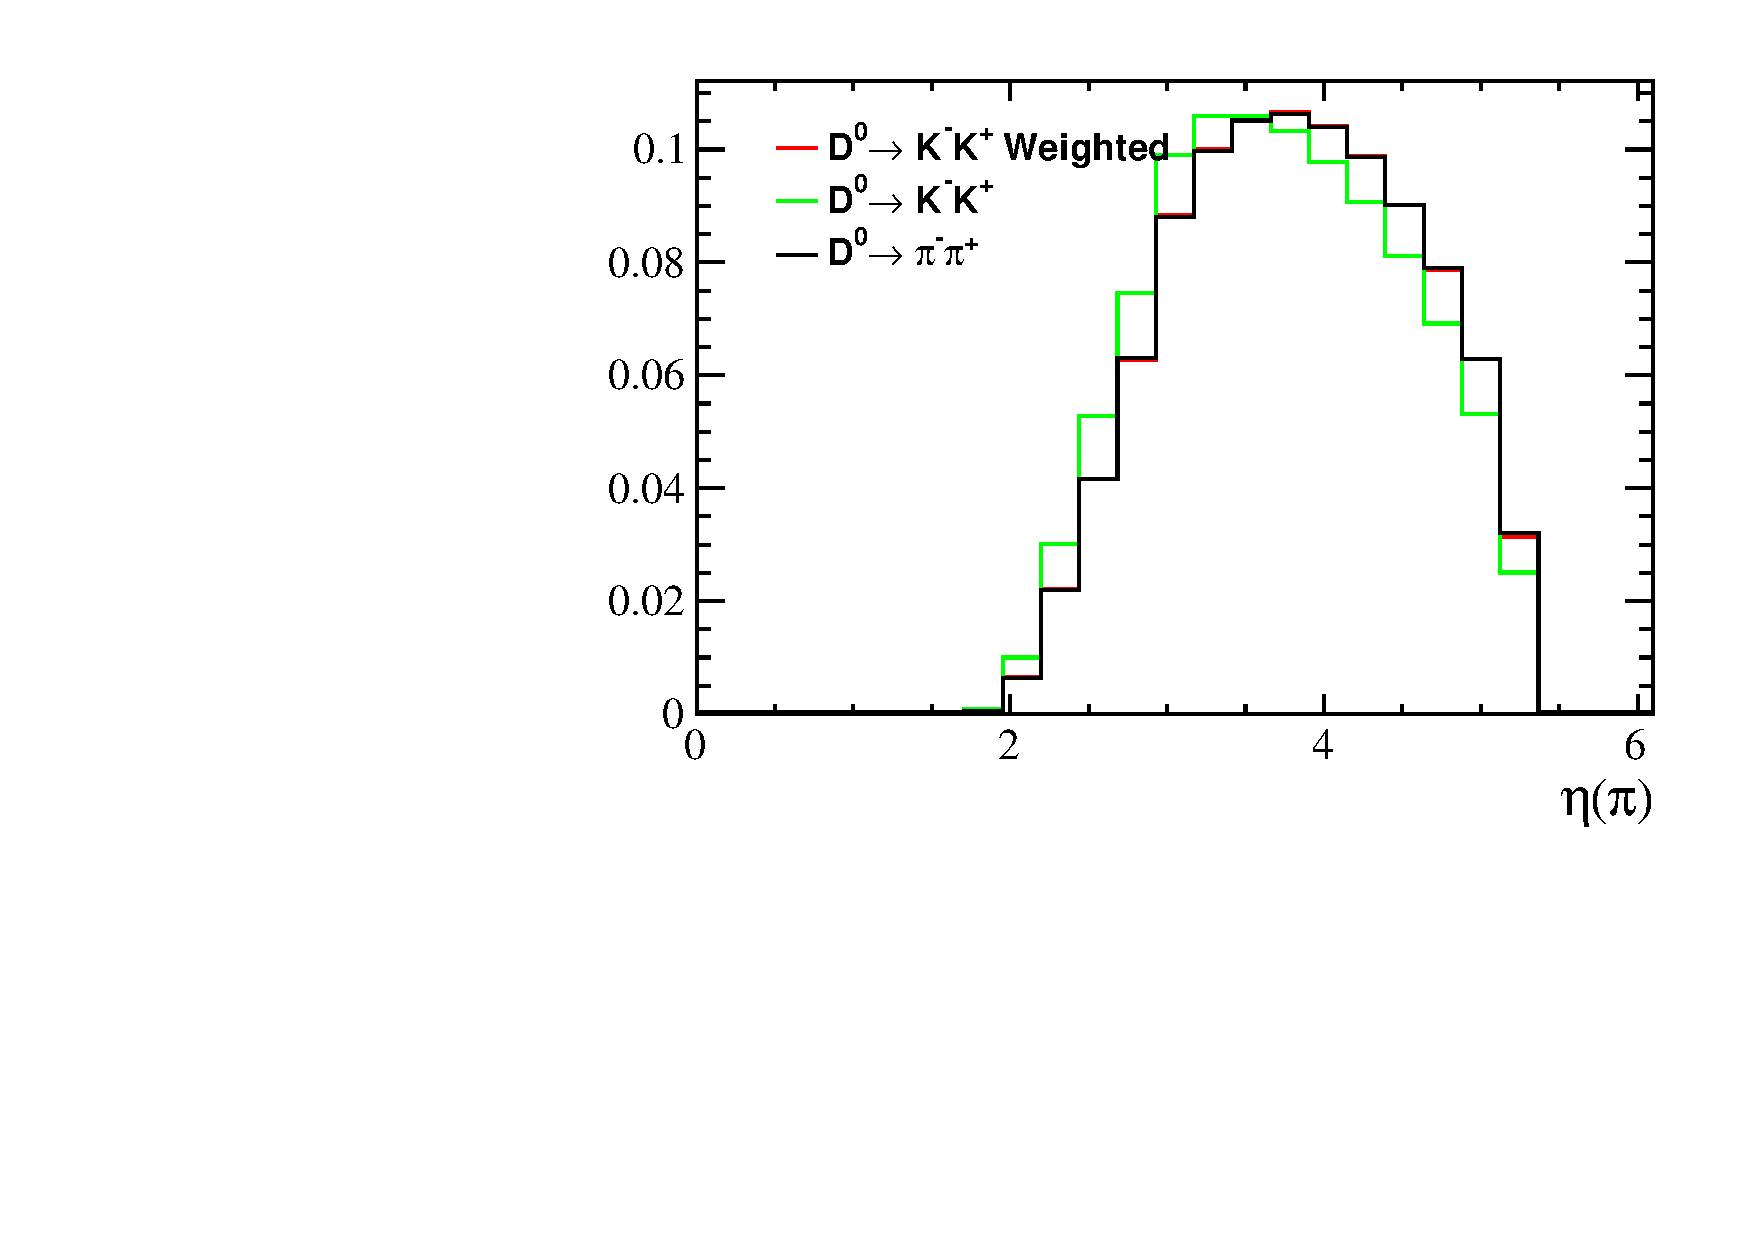
\includegraphics[width = 0.5\textwidth]{../../work/RapidSimAnalysis/WeightingFunction/Plots/sPi_eta_All.pdf}}
        \hfill
        \subfloat{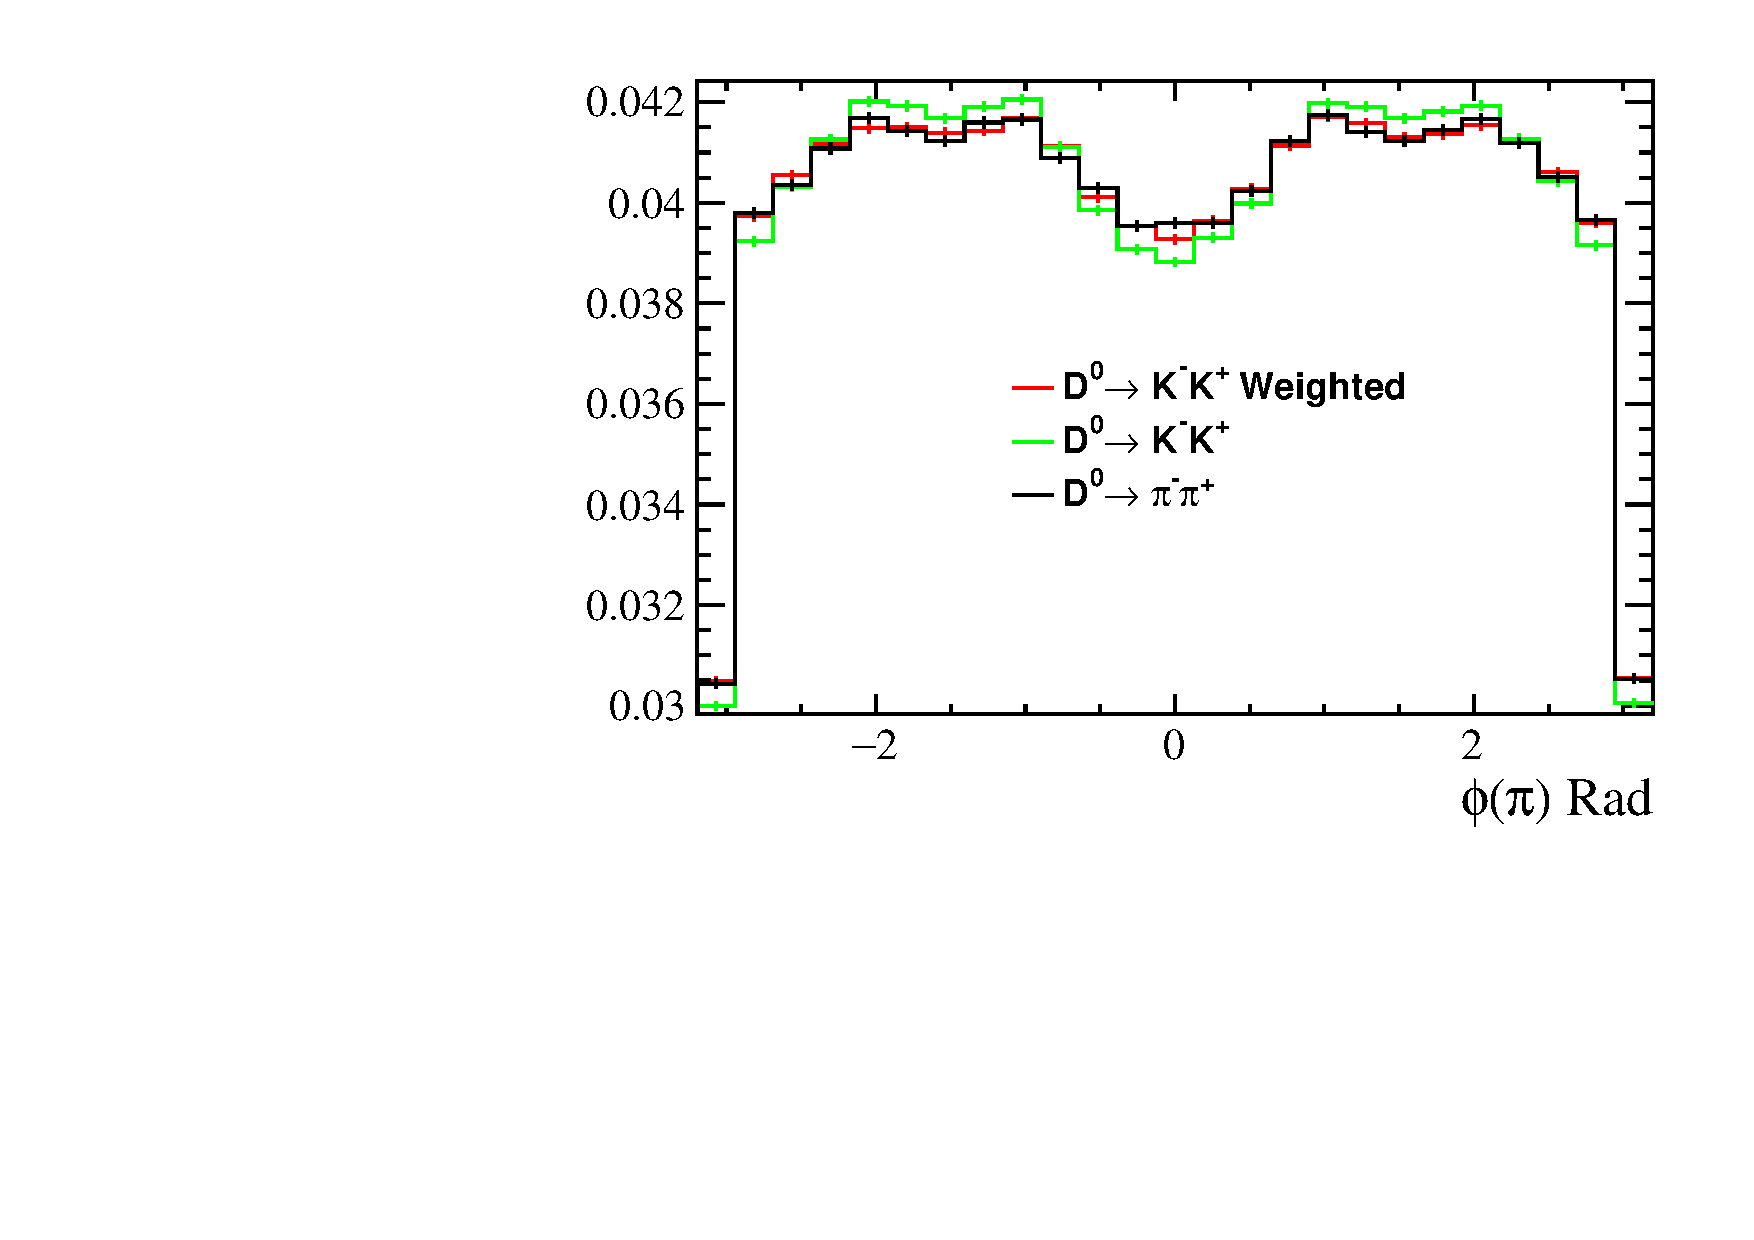
\includegraphics[width = 0.5\textwidth]{../../work/RapidSimAnalysis/WeightingFunction/Plots/sPi_phi_All.pdf}}
        \caption{We present the kinematic distributions $p_T$, $\eta$ and $\phi$ of $\pi_s$ for the two decay modes, before and after weighting.}
    \end{figure}

    As we can see, the kinematics of $D^0\to K^-K^+$ and $D^0\to \pi^-\pi^+$ samples match after the weighting which is expected, thus we conclude that the weighting is done correctly.
    
\end{document}